\documentclass{standalone}
\usepackage{tikz}
\usetikzlibrary{patterns}
\usetikzlibrary{positioning}
\usetikzlibrary{patterns, positioning}
\usetikzlibrary{shapes.misc}
\usepackage[outline]{contour}
\contourlength{1.5pt} 


\begin{document}
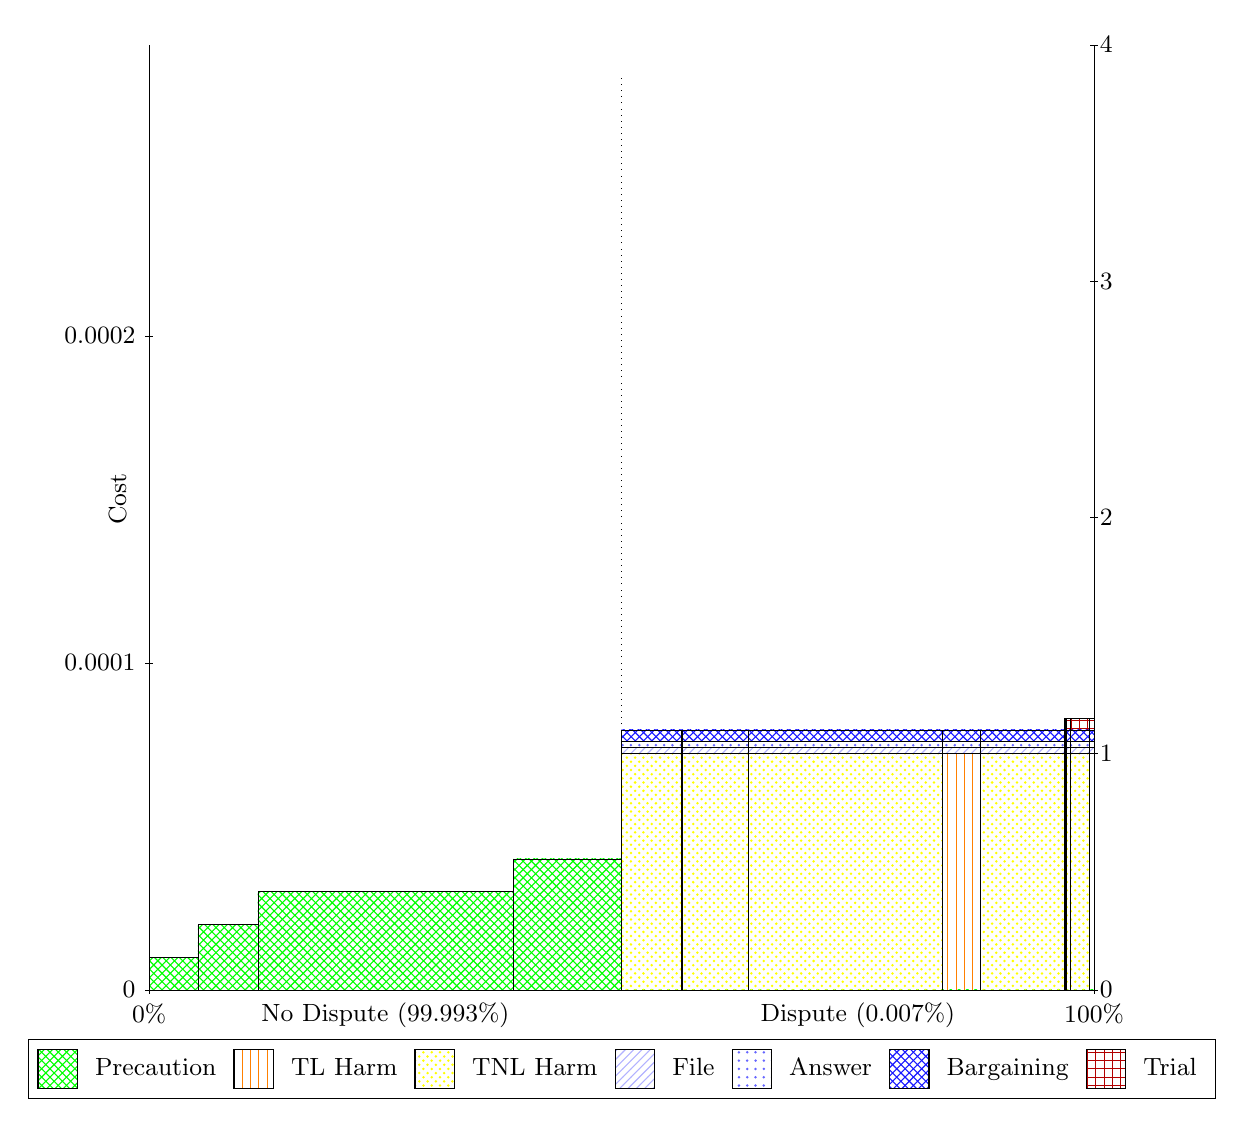
\begin{tikzpicture}
\draw[pattern=crosshatch, pattern color=green,draw=black,very thin] (1.5,2.5) rectangle (2.117,2.9153);
\draw[pattern=crosshatch, pattern color=green,draw=black,very thin] (2.117,2.5) rectangle (2.8801,3.3306);
\draw[pattern=crosshatch, pattern color=green,draw=black,very thin] (2.8801,2.5) rectangle (6.1199,3.7459);
\draw[pattern=crosshatch, pattern color=green,draw=black,very thin] (6.1199,2.5) rectangle (7.5,4.1612);
\draw[pattern=crosshatch, pattern color=green,draw=black,very thin] (7.5,2.5) rectangle (8.2605,2.5);
\draw[pattern=crosshatch dots, pattern color=yellow,draw=black,very thin] (7.5,2.5) rectangle (8.2605,5.5);
\draw[pattern=north east lines, pattern color=blue!30,draw=black,very thin] (7.5,5.5) rectangle (8.2605,5.575);
\draw[pattern=dots,  pattern color=blue!60,draw=black,very thin] (7.5,5.575) rectangle (8.2605,5.65);
\draw[pattern=crosshatch,      pattern color=blue!90,draw=black,very thin] (7.5,5.65) rectangle (8.2605,5.8);
\draw[pattern=crosshatch, pattern color=green,draw=black,very thin] (8.2605,2.5) rectangle (8.2669,2.5);
\draw[pattern=vertical lines, pattern color=orange,draw=black,very thin] (8.2605,2.5) rectangle (8.2669,5.5);
\draw[pattern=north east lines, pattern color=blue!30,draw=black,very thin] (8.2605,5.5) rectangle (8.2669,5.575);
\draw[pattern=dots,  pattern color=blue!60,draw=black,very thin] (8.2605,5.575) rectangle (8.2669,5.65);
\draw[pattern=crosshatch,      pattern color=blue!90,draw=black,very thin] (8.2605,5.65) rectangle (8.2669,5.8);
\draw[pattern=crosshatch, pattern color=green,draw=black,very thin] (8.2669,2.5) rectangle (9.1081,2.5001);
\draw[pattern=crosshatch dots, pattern color=yellow,draw=black,very thin] (8.2669,2.5001) rectangle (9.1081,5.5001);
\draw[pattern=north east lines, pattern color=blue!30,draw=black,very thin] (8.2669,5.5001) rectangle (9.1081,5.5751);
\draw[pattern=dots,  pattern color=blue!60,draw=black,very thin] (8.2669,5.5751) rectangle (9.1081,5.6501);
\draw[pattern=crosshatch,      pattern color=blue!90,draw=black,very thin] (8.2669,5.6501) rectangle (9.1081,5.8001);
\draw[pattern=crosshatch, pattern color=green,draw=black,very thin] (9.1081,2.5) rectangle (9.1119,2.5001);
\draw[pattern=vertical lines, pattern color=orange,draw=black,very thin] (9.1081,2.5001) rectangle (9.1119,5.5001);
\draw[pattern=north east lines, pattern color=blue!30,draw=black,very thin] (9.1081,5.5001) rectangle (9.1119,5.5751);
\draw[pattern=dots,  pattern color=blue!60,draw=black,very thin] (9.1081,5.5751) rectangle (9.1119,5.6501);
\draw[pattern=crosshatch,      pattern color=blue!90,draw=black,very thin] (9.1081,5.6501) rectangle (9.1119,5.8001);
\draw[pattern=crosshatch, pattern color=green,draw=black,very thin] (9.1119,2.5) rectangle (11.568,2.5001);
\draw[pattern=crosshatch dots, pattern color=yellow,draw=black,very thin] (9.1119,2.5001) rectangle (11.568,5.5001);
\draw[pattern=north east lines, pattern color=blue!30,draw=black,very thin] (9.1119,5.5001) rectangle (11.568,5.5751);
\draw[pattern=dots,  pattern color=blue!60,draw=black,very thin] (9.1119,5.5751) rectangle (11.568,5.6501);
\draw[pattern=crosshatch,      pattern color=blue!90,draw=black,very thin] (9.1119,5.6501) rectangle (11.568,5.8001);
\draw[pattern=crosshatch, pattern color=green,draw=black,very thin] (11.568,2.5) rectangle (12.054,2.5001);
\draw[pattern=vertical lines, pattern color=orange,draw=black,very thin] (11.568,2.5001) rectangle (12.054,5.5001);
\draw[pattern=north east lines, pattern color=blue!30,draw=black,very thin] (11.568,5.5001) rectangle (12.054,5.5751);
\draw[pattern=dots,  pattern color=blue!60,draw=black,very thin] (11.568,5.5751) rectangle (12.054,5.6501);
\draw[pattern=crosshatch,      pattern color=blue!90,draw=black,very thin] (11.568,5.6501) rectangle (12.054,5.8001);
\draw[pattern=crosshatch, pattern color=green,draw=black,very thin] (12.054,2.5) rectangle (13.118,2.5001);
\draw[pattern=crosshatch dots, pattern color=yellow,draw=black,very thin] (12.054,2.5001) rectangle (13.118,5.5001);
\draw[pattern=north east lines, pattern color=blue!30,draw=black,very thin] (12.054,5.5001) rectangle (13.118,5.5751);
\draw[pattern=dots,  pattern color=blue!60,draw=black,very thin] (12.054,5.5751) rectangle (13.118,5.6501);
\draw[pattern=crosshatch,      pattern color=blue!90,draw=black,very thin] (12.054,5.6501) rectangle (13.118,5.8001);
\draw[pattern=crosshatch, pattern color=green,draw=black,very thin] (13.118,2.5) rectangle (13.139,2.5);
\draw[pattern=crosshatch dots, pattern color=yellow,draw=black,very thin] (13.118,2.5) rectangle (13.139,5.5);
\draw[pattern=north east lines, pattern color=blue!30,draw=black,very thin] (13.118,5.5) rectangle (13.139,5.575);
\draw[pattern=dots,  pattern color=blue!60,draw=black,very thin] (13.118,5.575) rectangle (13.139,5.65);
\draw[pattern=crosshatch,      pattern color=blue!90,draw=black,very thin] (13.118,5.65) rectangle (13.139,5.8);
\draw[pattern=grid,            pattern color=red!70!black,draw=black,very thin] (13.118,5.8) rectangle (13.139,5.95);
\draw[pattern=crosshatch, pattern color=green,draw=black,very thin] (13.139,2.5) rectangle (13.144,2.5);
\draw[pattern=vertical lines, pattern color=orange,draw=black,very thin] (13.139,2.5) rectangle (13.144,5.5);
\draw[pattern=north east lines, pattern color=blue!30,draw=black,very thin] (13.139,5.5) rectangle (13.144,5.575);
\draw[pattern=dots,  pattern color=blue!60,draw=black,very thin] (13.139,5.575) rectangle (13.144,5.65);
\draw[pattern=crosshatch,      pattern color=blue!90,draw=black,very thin] (13.139,5.65) rectangle (13.144,5.8);
\draw[pattern=grid,            pattern color=red!70!black,draw=black,very thin] (13.139,5.8) rectangle (13.144,5.95);
\draw[pattern=crosshatch, pattern color=green,draw=black,very thin] (13.144,2.5) rectangle (13.193,2.5001);
\draw[pattern=crosshatch dots, pattern color=yellow,draw=black,very thin] (13.144,2.5001) rectangle (13.193,5.5001);
\draw[pattern=north east lines, pattern color=blue!30,draw=black,very thin] (13.144,5.5001) rectangle (13.193,5.5751);
\draw[pattern=dots,  pattern color=blue!60,draw=black,very thin] (13.144,5.5751) rectangle (13.193,5.6501);
\draw[pattern=crosshatch,      pattern color=blue!90,draw=black,very thin] (13.144,5.6501) rectangle (13.193,5.8001);
\draw[pattern=grid,            pattern color=red!70!black,draw=black,very thin] (13.144,5.8001) rectangle (13.193,5.9501);
\draw[pattern=crosshatch, pattern color=green,draw=black,very thin] (13.193,2.5) rectangle (13.201,2.5001);
\draw[pattern=vertical lines, pattern color=orange,draw=black,very thin] (13.193,2.5001) rectangle (13.201,5.5001);
\draw[pattern=north east lines, pattern color=blue!30,draw=black,very thin] (13.193,5.5001) rectangle (13.201,5.5751);
\draw[pattern=dots,  pattern color=blue!60,draw=black,very thin] (13.193,5.5751) rectangle (13.201,5.6501);
\draw[pattern=crosshatch,      pattern color=blue!90,draw=black,very thin] (13.193,5.6501) rectangle (13.201,5.8001);
\draw[pattern=grid,            pattern color=red!70!black,draw=black,very thin] (13.193,5.8001) rectangle (13.201,5.9501);
\draw[pattern=crosshatch, pattern color=green,draw=black,very thin] (13.201,2.5) rectangle (13.444,2.5001);
\draw[pattern=crosshatch dots, pattern color=yellow,draw=black,very thin] (13.201,2.5001) rectangle (13.444,5.5001);
\draw[pattern=north east lines, pattern color=blue!30,draw=black,very thin] (13.201,5.5001) rectangle (13.444,5.5751);
\draw[pattern=dots,  pattern color=blue!60,draw=black,very thin] (13.201,5.5751) rectangle (13.444,5.6501);
\draw[pattern=crosshatch,      pattern color=blue!90,draw=black,very thin] (13.201,5.6501) rectangle (13.444,5.8001);
\draw[pattern=grid,            pattern color=red!70!black,draw=black,very thin] (13.201,5.8001) rectangle (13.444,5.9501);
\draw[pattern=crosshatch, pattern color=green,draw=black,very thin] (13.444,2.5) rectangle (13.5,2.5001);
\draw[pattern=vertical lines, pattern color=orange,draw=black,very thin] (13.444,2.5001) rectangle (13.5,5.5001);
\draw[pattern=north east lines, pattern color=blue!30,draw=black,very thin] (13.444,5.5001) rectangle (13.5,5.5751);
\draw[pattern=dots,  pattern color=blue!60,draw=black,very thin] (13.444,5.5751) rectangle (13.5,5.6501);
\draw[pattern=crosshatch,      pattern color=blue!90,draw=black,very thin] (13.444,5.6501) rectangle (13.5,5.8001);
\draw[pattern=grid,            pattern color=red!70!black,draw=black,very thin] (13.444,5.8001) rectangle (13.5,5.9501);
\draw[black,very thin] (1.5,2.5) -- (1.5,14.5);
\node[font=\small,rotate=90,text=black, anchor=center] at (1.1, 8.7296) {Cost};
\draw[black,very thin] (1.45,2.5) -- (1.55,2.5);
\node[font=\small,text=black, anchor=east] at (1.45, 2.5) {0};
\draw[black,very thin] (1.45,6.6531) -- (1.55,6.6531);
\node[font=\small,text=black, anchor=east] at (1.45, 6.6531) {0.0001};
\draw[black,very thin] (1.45,10.806) -- (1.55,10.806);
\node[font=\small,text=black, anchor=east] at (1.45, 10.806) {0.0002};

\draw[black,dotted,very thin] (7.5,2.86) -- (7.5,14.14);
\draw[black,very thin] (13.5,2.5) -- (13.5,14.5);
\draw[black,very thin] (13.45,2.5) -- (13.55,2.5);
\node[font=\small,text=black, anchor=west] at (13.45, 2.5) {0};
\draw[black,very thin] (13.45,5.5) -- (13.55,5.5);
\node[font=\small,text=black, anchor=west] at (13.45, 5.5) {1};
\draw[black,very thin] (13.45,8.5) -- (13.55,8.5);
\node[font=\small,text=black, anchor=west] at (13.45, 8.5) {2};
\draw[black,very thin] (13.45,11.5) -- (13.55,11.5);
\node[font=\small,text=black, anchor=west] at (13.45, 11.5) {3};
\draw[black,very thin] (13.45,14.5) -- (13.55,14.5);
\node[font=\small,text=black, anchor=west] at (13.45, 14.5) {4};

\draw[black,very thin] (1.5,2.5) -- (13.5,2.5);
\draw[black,very thin] (1.5,2.45) -- (1.5,2.55);
\node[font=\small,text=black, anchor=north] at (1.5, 2.45) {0\%};
\draw[black,very thin] (13.5,2.45) -- (13.5,2.55);
\node[font=\small,text=black, anchor=north] at (13.5, 2.45) {100\%};

\node[font=\small,text=black,anchor=south] at (4.5, 1.9) {No\ Dispute\ (99.993\%)};
\node[font=\small,text=black,anchor=south] at (10.5, 1.9) {Dispute\ (0.007\%)};
\draw (7.5,2.5) node (B) {};
\begin{scope}[align=center]
\matrix[scale=0.5,draw=black,below=0.5cm of B,nodes={draw},column sep=0.1cm]{
\node[rectangle,draw,minimum width=0.5cm,minimum height=0.5cm,pattern=crosshatch, pattern color=green]{}; & \node[draw=none,font=\small,text=black]{Precaution}; &
\node[rectangle,draw,minimum width=0.5cm,minimum height=0.5cm,pattern=vertical lines, pattern color=orange]{}; & \node[draw=none,font=\small,text=black]{TL Harm}; &
\node[rectangle,draw,minimum width=0.5cm,minimum height=0.5cm,pattern=crosshatch dots, pattern color=yellow]{}; & \node[draw=none,font=\small,text=black]{TNL Harm}; &
\node[rectangle,draw,minimum width=0.5cm,minimum height=0.5cm,pattern=north east lines, pattern color=blue!30]{}; & \node[draw=none,font=\small,text=black]{File}; &
\node[rectangle,draw,minimum width=0.5cm,minimum height=0.5cm,pattern=dots,  pattern color=blue!60]{}; & \node[draw=none,font=\small,text=black]{Answer}; &
\node[rectangle,draw,minimum width=0.5cm,minimum height=0.5cm,pattern=crosshatch,      pattern color=blue!90]{}; & \node[draw=none,font=\small,text=black]{Bargaining}; &
\node[rectangle,draw,minimum width=0.5cm,minimum height=0.5cm,pattern=grid,            pattern color=red!70!black]{}; & \node[draw=none,font=\small,text=black]{Trial}; \\\\
};\end{scope}

\end{tikzpicture}
\end{document}